%%%%%%%%%%%%%%%%%%%%%%%%%%%%%%%%%%%%%%%%%%%%%%%%%%%%%%%%%%%%%%%%%%%%%%%%%%%%%%%%
% Diese Datei beinhaltet den eigentlichen Inhalt Ihrer Arbeit.
%
% Es bietet sich der Übersicht halber an, die einzelnen Abschnitte jeweils
% in eigene Dateien zu schreiben und mittels \input einzubinden.
% Eine mögliche Verzeichnisstruktur sähe entsprechend so aus:
%
%     thesis/
%     +- tex/
%     |  +- introduction.tex
%     |  +- motivation.tex
%     |  +- experiments.tex
%     |  |  ...
%     |  +- conclusion.tex
%     +- abstract.tex
%     +- contents.tex
%     +- thesis.tex
%%%%%%%%%%%%%%%%%%%%%%%%%%%%%%%%%%%%%%%%%%%%%%%%%%%%%%%%%%%%%%%%%%%%%%%%%%%%%%%%

\section{Einleitung}

Dies ist der Hauptteil Ihrer Arbeit.
Hier leiten Sie grob in das Thema ein, motivieren es und geben einen Ausblick
über das, was Sie in Ihrer Arbeit behandeln werden.

Der Inhalt der Vorlage ist mit Beispielen gefüllt, wie man \LaTeX{}
verwendet und traditionelle Stolpersteine vermeidet.
Lesen Sie die Vorlage gründlich.


\subsection{Makefile}

Im Wurzelverzeichnis finden Sie ein \texttt{Makefile}.
Über das Terminal können Sie die folgenden Befehle aufrufen,
wie in \cref{tab:make} beschrieben.


\begin{table}[h]
  \centering
  \caption{Übersicht der \texttt{Makefile}-Befehle.}%
  \label{tab:make}
  \begin{tabularx}{\textwidth}{lX}
    \toprule
    Befehl & Effekt \\
    \midrule
    \texttt{make} & Kompiliert das PDF und löscht aux-Files. \\
    \texttt{make clean} & Löscht das PDF und dazugehörige aux-Files. \\
    \texttt{make bibtool} & Sortiert \texttt{references.bib}
    und formatiert die Einträge einheitlich. \\
    \texttt{make watch} & Rekompiliert das PDF bei Änderungen und
    hält die Anzeige in Ihrem PDF-Betrachter aktuell. \\
    \bottomrule
  \end{tabularx}
\end{table}


\section{Referenzen und Zitationen}

In der Datei \texttt{references.bib} finden Sie bereits einige Quellen,
die Sie wahrscheinlich zitieren mögen,
wie z.B. die B Methode~\cite{abrial1996b,abrial2010modeling}
oder \textsc{ProB}~\cite{leuschel2003prob,leuschel2008prob}.
Beachten Sie den Artikel ``Common Errors in Bibliographies'' von John Owens.%
\footnote{\url{https://www.ece.ucdavis.edu/~jowens/biberrors.html}}
Zusätzliche, ausführlichere Informationen finden Sie auch in \cref{app:sec:bib}.


\subsection{Referenzen platzieren}

Sie platzieren Referenzen mit \texttt{\textbackslash{}cite{}}.
Diese sollten jeweils hinter dem Namen der zitierten Technik stehen,
oder hinter der zu belegenden Aussage.
Im Falle, dass sich ein gesamter Absatz auf eine einzelne Quelle bezieht,
genügt es die Referenz im ersten Satz anzugeben, solange vom Kontext klar ist,
dass der restliche Absatz sich ebenfalls auf die Quelle bezieht.
Referenzen sind nicht erst am Ende eines gesamten Absatzes zu platzieren.
Ebenso sind sie Teil des Satzes und stehen vor dem abschließenden Punkt.

\begin{itemize}
  \item Gut: \enquote{\textsc{ProB}~\cite{leuschel2003prob} is an
    animator, model checker, and constraint solver for the B method~\cite{abrial1996b}.
    The B method allows to specify, design, and code
    software systems as well as to perform formal proof of their properties.}
  \item Nicht gut: \enquote{\textsc{ProB} is an
    animator, model checker, and constraint solver for the B method~\cite{leuschel2003prob,abrial1996b}.
    The B method allows to specify, design, and code
    software systems as well as to perform formal proof of their properties.}
  \item Nicht gut: \enquote{\textsc{ProB} is an
    animator, model checker, and constraint solver for the B method
    The B method allows to specify, design, and code
    software systems as well as to perform formal proof of their properties.~\cite{leuschel2003prob,abrial1996b}}
\end{itemize}


\subsection{Über Literatur sprechen}

Obwohl die Referenzen innerhalb des Satzes stehen, sind sie keine Wörter.
Sie ersetzen somit nicht die explizite Nennung einer Quelle.
Sollte über ein bestimmtes Papier gesprochen werden, so ist dieses via
Autorennamen zu betiteln. Hierbei gilt:
\begin{itemize}
  \item Es sind nur die Nachnamen zu verwenden,
  \item hinter den Autorennamen ist die Referenz zu setzen,
    falls der Bezug unklar ist,
  \item ab drei oder mehr Autoren wird nur der Erstautor geführt, gefolgt von
    \enquote{et al.}.
\end{itemize}

So schreiben wir
\enquote{SICStus Prolog~\cite{carlsson1988sicstus} wurde von Carlson et al.\
  entwickelt}
oder
\enquote{Leuschel \& Butler~\cite{leuschel2003prob} haben einen Model Checker für die
  B-Methode~\cite{abrial1996b} entwickelt}.
Falsch hingegen ist es, eine Referenz als eigenständiges Wort zu nutzen, wie in
folgendem Negativbeispiel:
\enquote{In \cite{leuschel2003prob} wurde ein Model Checker für die B-Methode entwickelt}.



\section{Bilder und Tabellen}

Bilder und Tabellen sind per se wie von \LaTeX{} bekannt zu setzen.
Wichtig ist, dass sie ausnahmslos im Fließtext referenziert wurden.
Eine nichtreferenzierte Tabelle oder Abbildung kann ebenso ausgelassen werden.
Solche Querverweise werden in \cref{sec:references} besprochen.


\subsection{Bilder}%
\label{sec:figures}

\Cref{fig:initial-draft} ist eine exemplarische Abbildung, auf die an dieser
Stelle im Text verwiesen wird.
Stilistisch ist es meist empfehlenswert innerhalb der
\texttt{figure}-Umgebung ein \texttt{\textbackslash{}centering} zu setzen,
sodass der Inhalt zentriert wird.
In \cref{fig:hhu-logo} wird ein Beispiel der
\texttt{\textbackslash{}subfigure}-Umgebung aus dem
\texttt{\textbackslash{}subcaption}-Paket demonstriert.
Beide Teilabbildungen, \cref{fig:hhu-rgb,fig:hhu-bw},
sind individuell referenzierbar.

\begin{figure}[h]
  \centering
  \includegraphics[width=4cm]{fig/the.png}
  \caption{Initial thesis draft.}%
  \label{fig:initial-draft}
\end{figure}

\begin{figure}[h]
  \begin{subfigure}{.5\textwidth}
    \centering
    
\includegraphics[width=4cm]{fig/hhu-logo-rgb.pdf}
    \subcaption{in Farbe}%
    \label{fig:hhu-rgb}
  \end{subfigure}% <- Kommentarzeichen am Ende der Zeile ist wichtig!
  \begin{subfigure}{.5\textwidth}
    \centering
    
\includegraphics[width=4cm]{fig/hhu-logo-black.pdf}
    \subcaption{Schwarzweiß}%
    \label{fig:hhu-bw}
  \end{subfigure}% <- Kommentarzeichen am Ende der Zeile ist wichtig!
  \caption{Das neue HHU-Logo.}%
  \label{fig:hhu-logo}
\end{figure}


\subsection{Tabellen}%
\label{sec:tables}

Während bei Abbildungen die \texttt{\textbackslash{}caption}
in aller Regel unter dem Bild steht,
wird sie bei Tabellen typischer Weise darüber platziert, wie bei
\cref{table:truths} zu sehen.

\begin{table}[ht]
  \begin{center}
    \caption{Table of truths.}%
    \label{table:truths}
    \begin{tabular}{lr}
      \toprule
      Fakt                                & Wahrheitsgehalt \\
      \midrule
      booktabs-Tabellen sind hübscher     & 90 \%           \\
      Han Solo schoss zuerst              & 100 \%          \\
      Game of Thrones fand ein gutes Ende & 0 \%            \\
      \bottomrule
    \end{tabular}
  \end{center}
\end{table}

Es ist zu empfehlen, das Paket \texttt{booktabs} zur Formatierung der Tabellen
zu nutzen.
Dieses empfiehlt die Verwendung der Befehle
\texttt{\textbackslash{}toprule},
\texttt{\textbackslash{}midrule} und
\texttt{\textbackslash{}bottomrule},
und rät davon ab, vertikale Linien zu nutzen.
Vergleichen Sie \cref{tab:booktabs-yes,tab:booktabs-yesnt}.

\begin{table}
  \centering
  \caption{Vergleich von \LaTeX{}-Tabellen mit und ohne booktabs.}
  \begin{subtable}{.5\textwidth}
    \centering
    \subcaption{mit booktabs}%
    \label{tab:booktabs-yes}
    \begin{tabular}{lrr}
      \toprule
      Backend & Accuracy & F\textsubscript{1}-Score \\
      \midrule
      CLP(FD) & 0.947 & 0.966 \\
      Z3      & 0.919 & 0.797 \\
      \bottomrule
    \end{tabular}
  \end{subtable}%
  \begin{subtable}{.5\textwidth}
    \centering
    \subcaption{ohne booktabs}%
    \label{tab:booktabs-yesnt}
    \begin{tabular}{|l|r|r|}
      \hline
      Backend & Accuracy & F\textsubscript{1}-Score \\ \hline
      CLP(FD) & 0.947 & 0.966 \\ \hline
      Z3      & 0.919 & 0.797 \\ \hline
    \end{tabular}
  \end{subtable}%
\end{table}



\subsection{Plots}%
\label{sec:plot}

Sie können mithilfe von \texttt{tikz} und \texttt{pgfplots}
Graphen oder Bar Charts erstellen,
wie in \cref{fig:the-plot,fig:long-caption} der gezeigt ist.
Beachten Sie, dass die Vorlage die Cycle Lists
\texttt{hhubwcycle} (schwarzweiß) und \texttt{hhucolorcycle} bereit stellt,
welche die offiziellen HHU-Farben zur Darstellung der verschiedenen Graphen
verwendet.
Diese können in jeglichem \texttt{tikzplot} mittels der Option
\texttt{cycle list name=} gesetzt werden und stehen, je nach Druckeinstellung
innerhalb der PDF via \texttt{\textbackslash{}blackwhiteprint}
entweder automatisch auf \texttt{hhucolorcycle} oder \texttt{hhubwcycle}.

\begin{figure}[ht]
  \centering
  \begin{subfigure}{.5\textwidth}
    \centering
    \begin{tikzpicture}
      \begin{axis}[
        width=\textwidth,
        cycle list name=hhucolorcycle
      ]
        \foreach \y in {0,0.1,...,1} % Wiederholt \addplot mit jeweils anderem \y
          \addplot coordinates {
              ( 1, 3.0 -\y)
              ( 2, 3.25-\y)
              ( 3, 3.5 -\y)
              ( 4, 3.75-\y)
              ( 5, 4.0 -\y)
            };
      \end{axis}
    \end{tikzpicture}
    \subcaption{in den HHU-Farben}
  \end{subfigure}%
  \begin{subfigure}{.5\textwidth}
    \centering
    \begin{tikzpicture}
      \begin{axis}[
        width=\textwidth,
        cycle list name=hhubwcycle % <- Änderung auf schwarzweiß.
      ]
        \foreach \y in {0,0.1,...,1} % Wiederholt \addplot mit jeweils anderem \y
          \addplot coordinates {
              ( 1, 3.0 -\y)
              ( 2, 3.25-\y)
              ( 3, 3.5 -\y)
              ( 4, 3.75-\y)
              ( 5, 4.0 -\y)
            };
      \end{axis}
    \end{tikzpicture}
    \subcaption{in schwarzweiß}
  \end{subfigure}%
  \caption{A beautiful plot.}%
  \label{fig:the-plot}
\end{figure}

\begin{figure}[ht]
  \centering
  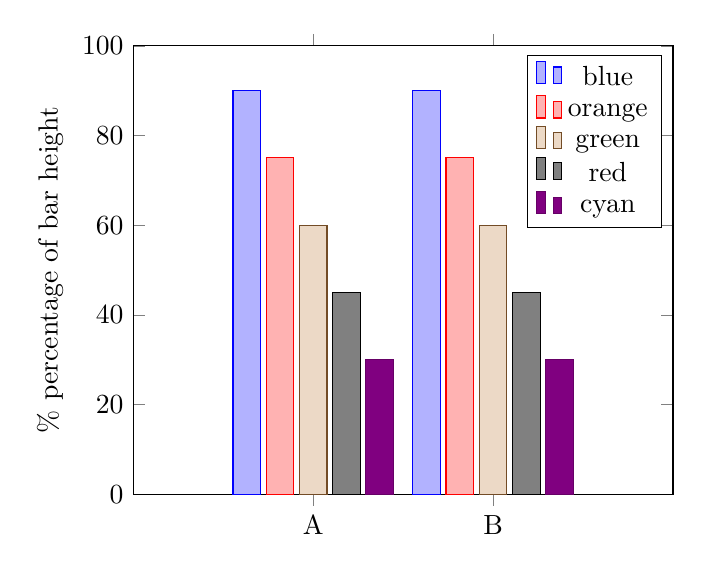
\begin{tikzpicture}
    \begin{axis}
      [
        ybar,
        xtick=data,
        enlarge x limits=1,
        symbolic x coords={A, B},
        ymin=0, ymax=100,
        ylabel={$\%$ percentage of bar height},
      ]
      \addplot coordinates {(A,90) (B, 90)};
      \addplot coordinates {(A,75) (B, 75)};
      \addplot coordinates {(A,60) (B, 60)};
      \addplot coordinates {(A,45) (B, 45)};
      \addplot coordinates {(A,30) (B, 30)};
      \legend{blue, orange, green, red, cyan}
    \end{axis}
  \end{tikzpicture}
  \caption[Bar plot with short version of caption for List of Figures]{%
    A really long caption title. This demonstrates how to describe stuff seen
    in the figure, like here, where we see a bar plot showing my favourite
    pies. Nah, actually it shows something completely different.
  }\label{fig:long-caption}
\end{figure}



\section{Querverweise}\label{sec:references}

Für Querverweise, wie zu
\cref{fig:initial-draft,fig:hhu-logo,fig:the-plot,fig:long-caption},
\cref{lst:hello-c,lst:hello-prolog}
oder \cref{alg:minimax}
stehen zwei Möglichkeiten zur Verfügung:
die \LaTeX{}-Standardvariante via \texttt{\textbackslash{}ref},
oder (eleganter) das \texttt{cleveref}-Paket.

Cleveref ermittelt automatisch, welche Art von Element referenziert wird
und fügt den entsprechenden Titel hinzu. Entsprechend sind die in
\cref{tab:cleveref} aufgeführten Beispiele äquivalent.

\begin{table}[ht]
  \centering
  \caption{Vergleich \texttt{\textbackslash{}ref} und \texttt{\textbackslash{}cref}.}%
  \label{tab:cleveref}
  \begin{tabularx}{\textwidth}{XX}
    \toprule
    \LaTeX{} & Darstellung \\
    \midrule
    \lstinline[language=tex]|Abbildung \\ref\{fig:logo\} zeigt das Logo.| &
      Abbildung \ref{fig:hhu-logo} zeigt das Logo. \\
    \lstinline[language=tex]|\\cref\{fig:logo\} zeigt das Logo.| &
      \cref{fig:hhu-logo} zeigt das Logo. \\
    \addlinespace
    \lstinline[language=tex]|Abbildungen \\ref\{fig:plot1\} und|
      \lstinline[language=tex]|\\ref\{plot2\} sind Graphen.| &
    Abbildungen \ref{fig:the-plot} und \ref{fig:long-caption} sind Graphen.\\
    \lstinline[language=tex]|\\Cref\{fig:plot1,plot2\} sind Graphen.| &
    \Cref{fig:the-plot,fig:long-caption} sind Graphen.\\
    \bottomrule
  \end{tabularx}
\end{table}



\section{Formeln}

\Cref{eq:example1} gibt eine referenzierbare Formel an,
während \cref{eq:example2} eine Formel darstellt, die länger ist, als die
Zeile zulässt.

\begin{equation}
  \label{eq:example1}
  2 = 1 + 1
\end{equation}

\begin{multline}
  \label{eq:example2}
  30 = 1 + 1 + 1 + 1 + 1 + 1 + 1 + 1 + 1 + 1 + 1 + 1 + 1 + 1 + 1 + 1 + 1 + 1 \\
      + 1 + 1 + 1 + 1 + 1 + 1 + 1 + 1 + 1 + 1 + 1 + 1
\end{multline}

In der zweizeiligen Gleichung
\begin{equation}
  \label{eq:mlp-stacking}
  \begin{split}
    \hat{y} & = f_2(f_1(x; W); V) \\
            & = f(x; W, V)
  \end{split}
\end{equation}
wurden die Gleichheitszeichen in beiden Zeilen direkt untereinander ausgerichtet
(mittels \texttt{\&} im Quelltext und der \texttt{split}-Umgebung).
Teilen wir \cref{eq:mlp-stacking}, welche den Forward Pass eines Neuronalen
Netzes darstellt,
in mehrere Schritte auf, so erhalten wir (mittels \texttt{align}-Umgebung)
\begin{align}
  a       & = W^\mathsf{T} x \label{eq:fp-act} \\
  h       & = g_1(a) \label{eq:fp-hidden} \\
  o       & = V^\mathsf{T} h \label{eq:fp-out} \\
  \hat{y} & = g_2(o) \label{eq:fp-pred}
  \,\text{,}
\end{align}
wobei \cref{eq:fp-act,eq:fp-hidden,eq:fp-out,eq:fp-pred} jeweils eine eigene
Referenznummer erhalten.


\section{Algorithmen}

Für Algorithmen kann das bereits inkludierte Paket \texttt{algorithmicx}
genutzt werden.
In \cref{alg:minimax} wird exemplarisch eine Implementierung des
Minimax-Algorithmus aufgeführt.
Beachten Sie, dass \cref{line:commented} kommentiert und referenzierbar ist.

\begin{algorithm}
  \caption{Determining the next action by Minimax}%
  \label{alg:minimax}
  \begin{algorithmic}[1]
    \Function{Minimax}{Game State Tree: $G^n$}
      \State bestValue \(\gets -\infty\)
      \State \(\mathit{bestAction} \gets \) NIL
      \ForAll{\(G^n_a \in S(G^n)\)}
        \State \(\mathit{value} = \) \Call{MinimaxValue}{\(G^n_a\), true}
        \If{\(\mathit{value} > \mathit{bestValue}\)}
          \Comment{Aktualisiere besten Wert}\label{line:commented}
          \State \(\mathit{bestValue} \gets \mathit{value}\)
          \State \(\mathit{bestAction} \gets a\)
        \EndIf
      \EndFor
      \State \Return \(\mathit{bestAction}\)
    \EndFunction
    \Statex
    \Function{MinimaxValue}{Game State Tree: $G^n$, Boolean: $\mathit{ourTurn}$}
      \If{\(D(G^n)=0\)}
        \State \Return \Call{Heuristic}{root(\(G^n\))}
      \ElsIf{\(\mathit{ourTurn}\)}
        \State \(\mathit{maxValue} \gets -\infty \)
        \ForAll{\(S \in S(G^n)\)}
          \State \(\mathit{newValue} \gets \) \Call{MinimaxValue}{\(S\), false}
          \State \(\mathit{maxValue} \gets
            \max(\mathit{newValue}, \mathit{maxValue})\)
        \EndFor
        \State \Return \(maxValue\)
      \Else
        \State \(minValue \gets +\infty \)
        \ForAll{\(S \in S(G^n)\)}
          \State \(\mathit{newValue} \gets \) \Call{MinimaxValue}{\(S\), true}
          \State \(\mathit{minValue} \gets
            \min(\mathit{newValue}, \mathit{minValue})\)
        \EndFor
        \State \Return \(minValue\)
      \EndIf
    \EndFunction
  \end{algorithmic}
\end{algorithm}


\section{Source Code Listings}

\Cref{lst:hello-c,lst:hello-python} zeigen ein `Hello World'-Programm,
je in C und Python.
\Cref{lst:hello-prolog} zeigt ein Prolog-Prädikat, welches eine Liste in zwei
Teile teilen kann.

\begin{lstlisting}[
  float, caption={Hello World in C.}, label={lst:hello-c}, language=C
]
#include <stdio.h>

int main(int argc, char[] *args){
  printf("Hello World!\n");
  // And done!
}
\end{lstlisting}

\begin{lstlisting}[
  float, caption={Totally minimal Hello World in Python.},
  label={lst:hello-python}, language=Python
]
def hello_world():
  print("Hello World"!)

if __name__ == "__main__":
  hello_world()
\end{lstlisting}

\begin{lstlisting}[
  float, caption={Prolog implementation of \texttt{split/4}},
  label={lst:hello-prolog}, language=Prolog
]
% Split list into two parts (length of first list given).
%
% ?- split([a,b,c,d,e,f,g,h,i,k], 3, L1, L2).
% L1 = [a,b,c]
% L2 = [d,e,f,g,h,i,k]
%
split(L, N, L1, L2) :-
  length(L1, N),
  append(L1, L2, L).
\end{lstlisting}


\section{Todonotes}

Es bietet sich an, während der Verschriftlichung Gebrauch von dem
\texttt{todonotes}-Package zu machen.\todo[]{Lernen, wie man mit todonotes umgeht.}

Abgesehen davon, dass es erlaubt die PDF mit offenen Todos zu annotieren,
sind sie ein guter Weg um potentziellen Korrekturlesern zu kommunizieren,
welche Teile ohnehin noch nicht ausgearbeitet sind.
Des Weiteren lässt sich mit
\texttt{\textbackslash{}listoftodos} eine Übersicht der noch offenen Todos
im Dokument anzeigen

\listoftodos

\todo[inline]{Lerne was man machen kann, wenn man einzeln stehende Todos braucht.}
\todo[inline]{Lerne ebenfalls, \texttt{\textbackslash missingfigure} zu nutzen.}
\todo[inline]{Verschaffung eines Überblicks der in der Vorlage inkludierten Pakete.}


\subsection{Missingfigure}

Mittels \texttt{\textbackslash{}missingfigure} lassen sich bereits Abbildungen
im PDF darstellen, die noch erstellt werden müssen. Dies ermöglicht bereits einen
ersten Eindruck, wie das Layout um die Abbildung herum aussehen wird,
wie \cref{fig:missing} exemplarisch zeigt.

\begin{figure}
  \centering
  \missingfigure{Plot is still to be done, but the results from the HPC are not
    yet available.}
  \caption{Finale Laufzeiten meiner unfassbar guten Auswertung.}%
  \label{fig:missing}
\end{figure}


\section{Häufige Fehler}

Der wohl häufigste Fehler, den neue \LaTeX-Nutzer machen, ist eine falsche
Verwendung von Anführungszeichen.
Um dem Vorzubeugen sowie konsistente Anführungszeichen zu nutzen,
empfehlen wir den Einsatz von \texttt{\textbackslash{}enquote}
aus dem bereits inkludierten \texttt{csquotes}-Pakt.
% Dieses erlaubt ebenfalls eine gezielte und automatische Unterscheidung
% zwischen den \foreignquote{english}{englischen} und
% \foreignquote{german}{deutschen} Anführungszeichen.
Wird hingegen, wie in der Programmierung üblich, \textquotedbl verwendet,
versucht \LaTeX{} daraus einen Umlaut zu erzeugen.
So wird beispielsweise \texttt{\textquotedbl{}a} zu ä.

\Cref{tab:quotes} gibt eine Übersicht über verschiedene Möglichkeiten
Anführungszeichen zu setzen und demonstriert die falsche Verwendung von
\textquotedbl.

\begin{table}[ht]
  \centering
  \caption{Demonstration von csquotes.}%
  \label{tab:quotes}
  \begin{tabularx}{\textwidth}{XX}
    \toprule
    \LaTeX{} & Darstellung \\
    \midrule
    \texttt{Ein \textquotedbl{}Wort\textquotedbl{} in \textquotedbl{}Anführungszeichen\textquotedbl{}} &
      Ein "Wort" in "Anführungszeichen" \\ \addlinespace
    \texttt{Ein \textbackslash{}glqq Wort
        in \textbackslash{}glq Anführungszeichen\textbackslash{}grq\textbackslash{}grqq}&
      Ein \glqq Wort in \glq Anführungszeichen\grq\grqq \\ \addlinespace
    \texttt{Ein \textbackslash{}enquote\{Wort
        in \textbackslash{}enquote\{Anführungszeichen\}}\} &
      Ein \enquote{Wort in \enquote{Anführungszeichen}} \\
    \bottomrule
  \end{tabularx}
\end{table}

\section{Conclusion}

Am Ende der Arbeit werden noch einmal die erreichten Ergebnisse
zusammengefasst und diskutiert.
